\section{The internals of the compiler}

A compiler, or ``the little black box that turns code into a program'', consists of several different parts: First of all, there's the source program which is the input to the compiler. The code is scanned so that a string of tokens can be created. These are then parsed forming an Abstract Syntax Tree (AST). A semantic analysis on the AST is performed, with the help of a symbol table, and the program is translated, optimized and finally the target code is generated. The process will be described to provide a little background knowledge of the compiler construction. 

Below is an illustration:

\begin{figure}[ht]
	\centering
		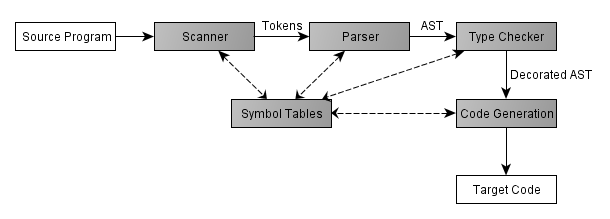
\includegraphics{img/compiler.png}
	\caption{Compiler}
	\label{fig:compiler}
\end{figure}


\subsection{The Scanner}

A scanner, sometimes referred to as a lexical analyzer or lexer, is the part of the compiler responsible for transforming characters from the source program into a stream of tokens, i.e. the elementary symbols that define the language syntax, and the symbols that the parser can work with.
It is very important to have a formal definition of the tokens so that lexical rules are clearly stated and followed.
For a simple syntax an ad hoc scanner can be constructed to find the tokens, but for more complex syntaxes a scanner generator may be a time-saving choice.
When the scanner scans tokens they have two components: a type and a semantic value, the first indicating the token's membership in the terminal alphabet, the latter providing information about the token, if any is needed.
An example where the semantic value may not be needed is a terminal like "plus" in a simple calculator language. The terminal can only correspond to one token, namely the +. However for, say, an identifier it is important to have a semantic value to denote which identifier this is.
When the scanner tries to determine what kind of token is being scanned it will have a method that looks ahead, without removing the characters. Several algorithms for determining membership in the terminal alphabet can be employed, and often the scanner will also be instructed to skip certain parts of the code, like blanks and comment sections.

\subsection{The Parser}

The parser is the part of the compiler that makes sure that the tokens generated by the scanner from the source code conforms to the syntactical structure defined by the grammar of the language. The result is an AST. 

There are several ways to handle the parser problem, i.e. the problem of creating the parse tree from the token stream. Some parsers create the tree from the root to the leaves, called top-down or LL parsing, others create the tree from the leaves up, called bottom-up or LR parsing. LL-parsers are, in theory, weaker than LR-parsers, but they are simple and often constructed anyway.

The LL(k)-parser works by looking ahead at the next k tokens to decide which production to use. Generally as low a value of k as possible is preferable. 

The LR(k)-parser reads tokens until only one production rule applies. For each node it then checks if the node and its children can generate a parent node.

\subsection{Type Checking}

The semantic analysis creates what is called a decorated AST. What it does is check what is called the static semantics of each node. This means that each node is meaningful and legal with regards to types, identifier declaration etc. for the source language. If it is, the node is decorated with  type information. Should an error be discovered, an error message is sent out.

\subsection{Translator}

Once the AST has been verified, the meaning of the AST should be implemented. This can be done using IR code, which makes sure that e.g. loops loop. Many compiler however generate the target code directly from the AST instead of via IR code.

\subsection{The Symbol Table}

The symbol table is a central table accessible from all compiler phases which contains information that is associated with identifiers. When an identifier is declared, its information is stored in the symbol table, so that the next time it is used it can be retrieved from the table. This is used in type checking.

\subsection{The Optimizer}

Optimization of the code means analysing and transforming the IR code, so that it does the same, but is more efficient thus speeding up the target code. This is a quite complex phase, which, especially if a high level of optimization is chosen, will take longer than if no optimization is chosen.

\subsection{The Code Generator}
This is where the target code is generated, either directly from the decorated AST or from the IR code. This phase need detailed knowledge the target machine, e.g. register allocation, code scheduling and so on. This phase is often coded by hand instead of using a tool, and a good code generator requires many special cases to be considered.